\documentclass[margin=5mm]{standalone}
\usepackage[dvipsnames]{xcolor}
\usepackage{pgfplots}
\usepackage{tikz}
\usepackage[tikz]{ocgx2}

\pgfplotsset{compat=1.18}
\begin{document}

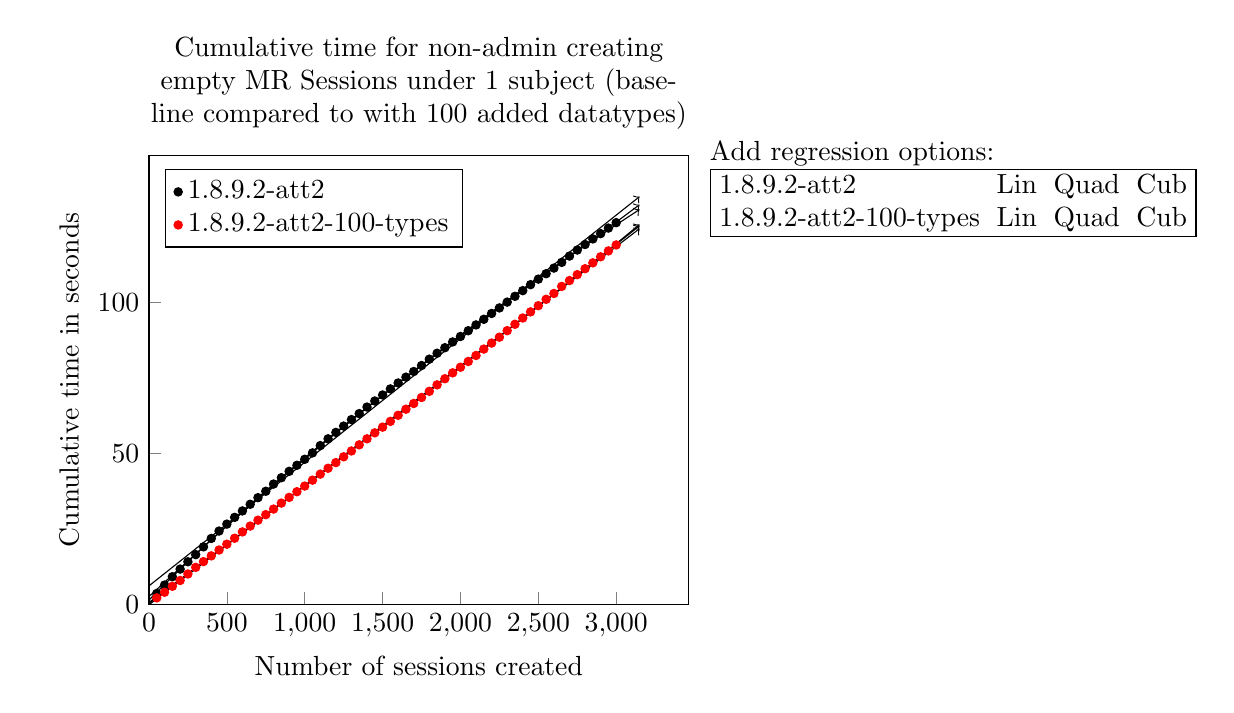
\begin{tikzpicture}
    \begin{axis}[
        align = center,
        legend pos = north west,
        legend cell align = left,
        xlabel = Number of sessions created,
        ylabel = Cumulative time in seconds,
        xtick pos = left,
        ytick pos = left,
        scaled ticks = false,
        xmin = 0,
        ymin = 0,
        title = {Cumulative time for non-admin creating empty MR Sessions under 1 subject (baseline compared to with 100 added datatypes)},
        title style = {text width = 0.8\textwidth},
        legend entries={\switchocg{1.8.9.2-att2}{1.8.9.2-att2},\switchocg{1.8.9.2-att2-100-types}{1.8.9.2-att2-100-types}}]
        \begin{scope}[ocg = {ref = 1.8.9.2-att2-Lin, status = invisible}]
            \plot[domain=0:3150,->,forget plot] (\x,{6.05523954802257957652500408585183322429656982421875 + 0.040913853848291194259534364618957624770700931549072265625*(\x)^1});
        \end{scope}
        \begin{scope}[ocg = {ref = 1.8.9.2-att2-Quad, status = invisible}]
            \plot[domain=0:3150,->,forget plot] (\x,{2.50236832261831576573740676394663751125335693359375 + 0.04779037880068652544007790083924192003905773162841796875*(\x)^1 + -0.00000225459834504764794330979038594620078583830036222934722900390625*(\x)^2});
        \end{scope}
        \begin{scope}[ocg = {ref = 1.8.9.2-att2-Cub, status = invisible}]
            \plot[domain=0:3150,->,forget plot] (\x,{1.3788624011811716485453871428035199642181396484375 + 0.052036262275033960678083388984305202029645442962646484375*(\x)^1 + -0.000005706229440092651597634353100030324412728077732026576995849609375*(\x)^2 + 0.0000000007544548841628418949285000524493903506506597977931960485875606536865234375*(\x)^3});
        \end{scope}
        \begin{scope}[ocg = {ref = 1.8.9.2-att2, status = visible}]
            \addplot[
                only marks,
                color = black,
                mark = *,
                mark size = 1.5 pt
            ]coordinates {(50,3.528)(100,6.314)(150,9.081)(200,11.613)(250,14.036)(300,16.39)(350,18.976)(400,21.749)(450,24.202)(500,26.496)(550,28.735)(600,30.864)(650,33.066)(700,35.26)(750,37.371)(800,39.768)(850,41.855)(900,43.977)(950,45.973)(1000,47.962)(1050,50.082)(1100,52.491)(1150,54.744)(1200,56.863)(1250,58.957)(1300,61.099)(1350,63.084)(1400,65.256)(1450,67.261)(1500,69.247)(1550,71.264)(1600,73.226)(1650,75.158)(1700,77.022)(1750,79.004)(1800,81.112)(1850,83.075)(1900,84.901)(1950,86.817)(2000,88.623)(2050,90.528)(2100,92.445)(2150,94.307)(2200,96.239)(2250,98.071)(2300,99.999)(2350,101.916)(2400,103.799)(2450,105.763)(2500,107.607)(2550,109.405)(2600,111.264)(2650,113.151)(2700,115.237)(2750,117.233)(2800,119.067)(2850,120.92)(2900,122.666)(2950,124.511)(3000,126.302)};
        \end{scope}
        \begin{scope}[ocg = {ref = 1.8.9.2-att2-100-types-Lin, status = invisible}]
            \plot[domain=0:3150,->,forget plot] (\x,{-0.2184638418079156985118771672205184586346149444580078125 + 0.039536544595721034855984044042997993528842926025390625*(\x)^1});
        \end{scope}
        \begin{scope}[ocg = {ref = 1.8.9.2-att2-100-types-Quad, status = invisible}]
            \plot[domain=0:3150,->,forget plot] (\x,{0.56965967270601203242819110528216697275638580322265625 + 0.038011144245048915368823116978092002682387828826904296875*(\x)^1 + 0.000000500131262515448338584430655606727356143892393447458744049072265625*(\x)^2});
        \end{scope}
        \begin{scope}[ocg = {ref = 1.8.9.2-att2-100-types-Cub, status = invisible}]
            \plot[domain=0:3150,->,forget plot] (\x,{0.26286986373002518835306773326010443270206451416015625 + 0.0391705451482173561128519168050843290984630584716796875*(\x)^1 + -0.00000044238735185007930667078841942274625154141176608391106128692626953125*(\x)^2 + 0.00000000020601499767552511590588936788684577827712729458653484471142292022705078125*(\x)^3});
        \end{scope}
        \begin{scope}[ocg = {ref = 1.8.9.2-att2-100-types, status = visible}]
            \addplot[
                only marks,
                color = red,
                mark = *,
                mark size = 1.5 pt
            ]coordinates {(50,2.079)(100,3.935)(150,5.917)(200,7.835)(250,9.985)(300,12.174)(350,14.094)(400,15.993)(450,17.927)(500,19.851)(550,21.828)(600,23.924)(650,25.86)(700,27.804)(750,29.625)(800,31.481)(850,33.46)(900,35.344)(950,37.23)(1000,39.096)(1050,41.049)(1100,43.052)(1150,44.989)(1200,46.867)(1250,48.793)(1300,50.718)(1350,52.75)(1400,54.745)(1450,56.718)(1500,58.601)(1550,60.513)(1600,62.534)(1650,64.546)(1700,66.437)(1750,68.421)(1800,70.464)(1850,72.606)(1900,74.627)(1950,76.579)(2000,78.433)(2050,80.342)(2100,82.33)(2150,84.451)(2200,86.431)(2250,88.381)(2300,90.552)(2350,92.661)(2400,94.738)(2450,96.764)(2500,98.813)(2550,100.929)(2600,102.859)(2650,105.19)(2700,107.129)(2750,109.087)(2800,111.054)(2850,113.001)(2900,115.014)(2950,116.952)(3000,118.924)};
        \end{scope}
    \end{axis}
    \begin{scope}
        \addtolength{\tabcolsep}{-0.3em}
        \node [below right, shape=rectangle, align=left](regressiontable) at (7,6) {
            Add regression options: \\
            \begin{tabular}{|llll|}
                \hline
                1.8.9.2-att2 & \switchocg{1.8.9.2-att2-Lin}{Lin} & \switchocg{1.8.9.2-att2-Quad}{Quad} & \switchocg{1.8.9.2-att2-Cub}{Cub} \\
                1.8.9.2-att2-100-types & \switchocg{1.8.9.2-att2-100-types-Lin}{Lin} & \switchocg{1.8.9.2-att2-100-types-Quad}{Quad} & \switchocg{1.8.9.2-att2-100-types-Cub}{Cub} \\
                \hline
            \end{tabular}
        };
    \end{scope}
\end{tikzpicture}

\end{document}